\documentclass[landscape]{exam}

\usepackage{2in1, lscape} 
\usepackage{units} 
\usepackage[fleqn]{amsmath}
\usepackage{float}
\usepackage{mdwlist}
\usepackage{booktabs}
\usepackage{caption}
\usepackage{fullpage}
\usepackage{enumerate}
\usepackage{graphicx}
\usepackage{parskip}

\printanswers

\everymath{\displaystyle}

\printanswers

\title{Statistics \\ Week Thirteen}
\date{\today}
\author{}

\begin{document}

  \maketitle
  \tableofcontents

  \section{Product Rule}

  For independent events:
  \[
    P(\text{A and B}) = P(A) P(B)
  \]

  For dice, the probability of getting a pair of 6s is:
  \begin{itemize}
    \item 36 possible outcomes
    \item only 1 of these outcomes is a pair of 6s
    \item $\frac{1}{6} \cdot \frac{1}{6} = \frac{1}{36}$
  \end{itemize}

  independence:
  \begin{itemize*}
    \item outcome of A doesn't influence B
    \item dice and roulette are independent
    \item drawing cards without replacement isn't--cards already drawn are gone
      from the deck
  \end{itemize*}

  \section{Data Dredging}
  Suppose 
  \begin{itemize}
    \item database of 20,000 men.
    \item 1 out of 10,000 men will match DNA by chance
    \item search DB and find match
  \end{itemize}

  What is the probability that the match is guilty?

  \begin{solution}
    The probability that any one person matches is independent of the
    probability of anybody else matching.

    The probability that nobody matches is
    \[
      0.9999^{20,000} \approx 0.14
    \]

    The probability that somebody matches:
    \[
      1 - 0.1353 \approx 0.86
    \]
  \end{solution}

  \section{Addition Rule}

  \[
    P(\text{A or B}) = P(A) + P(B) - P(\text{A and B})
  \]

  \begin{itemize*}
    \item if $P(A and B) = 0$, events are {\em disjoint} or {\em mutually
      exclusive}
    \item for disjoint events, if A occurs B can't occur
    \item draw Venn diagram to explain why subtracting $P(\text{A and B})$ is
      necessary
  \end{itemize*}

  examples:
  \begin{itemize*}
    \item red cars, compact cars, red compact cars
    \item people with beards, people with mustaches, people with both
  \end{itemize*}

  \section{Independence vs. Disjoint}
  \begin{itemize*}
    \item two independent events may both happen. event one has no effect on
      event two.

    \item to disjoint events can never both happen. if event one happens, event
      two can't happen

  \end{itemize*}

  \section{Sally Clark}

  \subsection{Trial}
  \begin{itemize*}
    \item two children died unexplained deaths (SIDS)
    \item probability of SIDS 1 in 1300
    \item for Sally Clark's family (affluent non-smokers) probability is 1 in
      8543.
    \item overall probability is:
      \[
        \frac{1}{8543^2} \approx \frac{1}{73,000,000}
      \]

    \item with 700,000 births per year, the chance of a double SIDS happening at
      least once in 100 years is:
      \[
        1 - (1 - 1/8543^2)^(700000 * 100) \approx 0.62
      \]

      This sort of event will only happen about once in every hundred years.
  \end{itemize*}

  \subsection{Problems}

  The prosecution ignored factors that make Sally's family more likely for
  SIDS. Both of Sally's kids were boys and boys are more likely to die from
  SIDS.

  SIDS depends on genetic and environmental factors. If a family has one SIDS
  death, the chance of a second one is approximately 1 in 130, not 1 in 1300.

  The ``once in a hundred years'' calculation used the high number (8543)
  which was for a small subset of a population, but then used the whole
  population.

  With these corrections, the probability of double SIDS would be about:
  \[
    \frac{1}{1300} \cdot \frac{1}{130} \approx \frac{1}{169000} 
  \]

  With 700,000 births a year, the chance of a double-SIDS event in one year is
  about:
  \[
    1 - (1 - 1/169000)^(700000) \approx 0.98
  \]

  \section{Conditional Probability}

  \subsection{Definitions}
  \begin{align*}
    P(\text{A and B}) & = P(A) P(B | A) \\
    P(B) P(A | B)     & = P(A) P(B | A) \\
    P(A | B)          & = \frac{P(A) P(B | A)}{P(B)} \\
                      % & = P(B | A) \cdot \frac{P(A)}{P(B)} \\
                      & = \frac{P(\text{A and B})}{P(B)} \\
  \end{align*}

  \begin{table}[H]
    \begin{tabular}[H]{lrrr}
      \toprule
      species & white & black & total\\
      \midrule
      dog     & 30    & 70    & 100\\
      cat     & 25    & 25    & 50\\
      \midrule
      total   & 45    & 105   & 150\\
      \bottomrule
    \end{tabular}
  \end{table}

  \begin{table}[H]
    \begin{tabular}{rlrrr}
      \toprule
        & species & white  & black  & (all) \\
      \midrule
      1 & dog     & 0.2000 & 0.4667 & 0.6667 \\
      2 & cat     & 0.1667 & 0.1667 & 0.3333 \\
      \midrule
      3 & (all)   & 0.3667 & 0.6333 & 1.0000 \\
      \bottomrule
    \end{tabular}
  \end{table}

  \begin{table}[ht]
    \begin{tabular}{rllr}
      \toprule
         & species & color & proportion \\
      \midrule
      1  & dog     & white & 0.3000 \\
      2  & dog     & black & 0.7000 \\
      \midrule
      3  & cat     & white & 0.5000 \\
      4  & cat     & black & 0.5000 \\
      \bottomrule
    \end{tabular}
  \end{table}

  \begin{table}[ht]
    \begin{tabular}{rllr}
      \toprule
         & color & species & proportion \\
      \midrule
      1  & white & dog     & 0.5455 \\
      2  & white & cat     & 0.4545 \\
      \midrule
      3  & black & dog     & 0.7368 \\
      4  & black & cat     & 0.2632 \\
      \bottomrule
    \end{tabular}
  \end{table}

  What's the probability of a randomly selected animal being a black dog:
  \[
    \frac{70}{150} \approx 0.4667 \\
  \]

  \begin{align*}
    P(\text{black dog}) & = P(\text{dog}) \cdot P(\text{black } | \text{ dog}) \\
                        & = 0.6667 \cdot 0.7 \\
                        & \approx 0.4666 \\
                        \\
    P(\text{black dog}) & = P(\text{black}) \cdot P(\text{dog } | \text{ black}) \\
                        & = 0.6333 \cdot 0.7368 \\
                        & \approx 0.4666 \\
  \end{align*}

  \begin{align*}
    P(\text{black } | \text{ dog}) & = \frac{P(\text{black dog})}{P(\text{dog})} \\
                                   & \approx \frac{0.4667}{0.6667} \\
                                   & = 0.7 \\
  \end{align*}

  \begin{align*}
    P(\text{dog } | \text{ black}) & = \frac{P(\text{black dog})}{P(\text{black})} \\
                                   & \approx \frac{0.4667}{0.7} \\
                                   & = 0.6667 \\
  \end{align*}

  \subsection{Sally Clark Appeal}
  The probability of a double SIDS event is irrelevant. The alternative
  explanation for the evidence is double infant murder, which is even less
  likely that double SIDS. 
  
  The interesting probability is the conditional probability of Clark being
  innocent given the evidence.

  Since double infant murder is so rare, it's hard to get a good estimate of its
  frequency. The best estimate is that double murder is about 9 times less
  likely than double SIDS.

  \begin{align*}
    P(\text{double SIDS}) & = \frac{1}{8543 \cdot 132} \\
                            & \approx \frac{1}{125,000} \\
    P(\text{double murder}) & = \frac{1}{9 \cdot 8543 \cdot 132} \\
                            & \approx \frac{1}{1,128,000} \\
  \end{align*}

  \begin{align*}
    P(I | E) & = \frac{P(\text{I and E})}{P(E)} \\
             & = \frac{P(\text{double murder})}{P(\text{double murder or double SIDS})} \\
             & = \frac{\cfrac{1}{125,000}}{\cfrac{1}{125,000} + \cfrac{1}{1,128,000}} \\
             & \approx 0.9 \\
  \end{align*}

  Even this didn't get Sally out of prison. Her third appeal succeeded because
  they reviewed the medical records more carefully and found the actual cause of
  death for the second baby was an infection that had gone undetected.

  \subsection{OJ Case}
  Prosecutors said that there is a natural progression from abuse to murder.

  Defense countered with 
  \begin{itemize*}
    \item 14,000,000 women battered annually by spouse or boyfriend
    \item 1,432 of these, or 1 in 2,500 murdered by spouse
    \item chance of OJ having murdered Nicole only 1 in 2,500
    \item what is this ``natural progression'' crap?
  \end{itemize*}

  Prosecution should have countered with conditional probability. Murder by
  spouse is very rare, but murder by someone other than spouse is even more
  rare. Only about 160 battered spouses were murdered by someone other than
  the batterer.

  Probability of non-spouse murder of abused spouse:
  \[
    \frac{160}{14,000,000} \approx \frac{1}{87,500}
  \]

  Probability of abused spouse getting murdered:
  \[
    \frac{160 + 1432}{14,000,000} \approx \frac{1}{87,500} 
      \approx \frac{1}{8800}
  \]

  \begin{align*}
    P(I | E) & = \frac{P(\text{I and E})}{P(E)} \\
             & = \frac{P(\text{someone else guilty})}{P(\text{murdered})} \\
             & = \frac{\cfrac{1}{87,500}}{\cfrac{1}{8800}} \\
             & \approx 0.1 \\
  \end{align*}
  




  \section{Tree Diagram}
  \subsection{Test for Disease}

  \begin{itemize*}
    \item test 99.9999\% accurate
    \item no false negatives (everyone with disease tests positive)
    \item 1 out of 100,000 people have disease
    \item 175,000,000 people in US
  \end{itemize*}

  If test is administered to all people in US, what percentage of the people
  with positive results on test actually have disease?


  \begin{solution}
    level one:
    \begin{itemize*}
      \item 0.0001 have disease
      \item 0.99999 don't have disease
    \end{itemize*}

    level two: test positive/negative. 
    \begin{itemize*}
      \item Have the disease and test positive: 1,750
      \item Have the disease and test negative: 0
      \item Don't have the disease and test positive: 17,500
      \item Don't the disease and test negative: 174,980,750
    \end{itemize*}

    percentage of people who tested positive who have the disease:
    \[
      \frac{1,750}{19,250} \approx 9\%
    \]

  \end{solution}

  \subsection{Investment Decision}
  Expected value can also help us untangle complex decisions that involve many
  contingencies at different points in time. 

  Suppose a friend of yours has asked you to invest \$1 million in a research
  venture examining a new cure for male pattern baldness. You would probably ask
  what the likelihood of success will be; you’ll get a complicated answer. This
  is a research project, so there is only a 30 percent chance that the team will
  discover a cure that works. If the team does not find a cure , you will get
  \$250,000 of your investment back, as those funds will have been reserved for
  taking the drug to market (testing, marketing, etc.) Even if the researchers
  are successful, there is only a 60 percent chance that the U.S . Food and Drug
  Administration will approve the new miracle baldness cure as safe for use on
  humans. Even then, if the drug is safe and effective, there is a 10 percent
  chance that a competitor will come to market with a better drug at about the
  same time, wiping out any potential profits. If everything goes well---the drug
  is safe, effective, and unchallenged by competitors---then the best estimate
  on the return on your investment is \$ 25 million. 

  Should you make the investment? 

  % This seems like a muddle of information. The potential payday is huge— 25 times
  % your initial investment— but there are so many potential pitfalls.  A decision
  % tree can help organize this kind of information and— if the probabilities
  % associated with each outcome are correct— give you a probabilistic assessment of
  % what you ought to do. The decision tree maps out each source of uncertainty and
  % the probabilities associated with all possible outcomes. The end of the tree
  % gives us all the possible payoffs and the probability of each. If we weight each
  % payoff by its likelihood, and sum all the possibilities, we will get the
  % expected value of this investment opportunity. As usual, the best way to
  % understand this is to take a look.

  \begin{figure}[H]
    \centering
    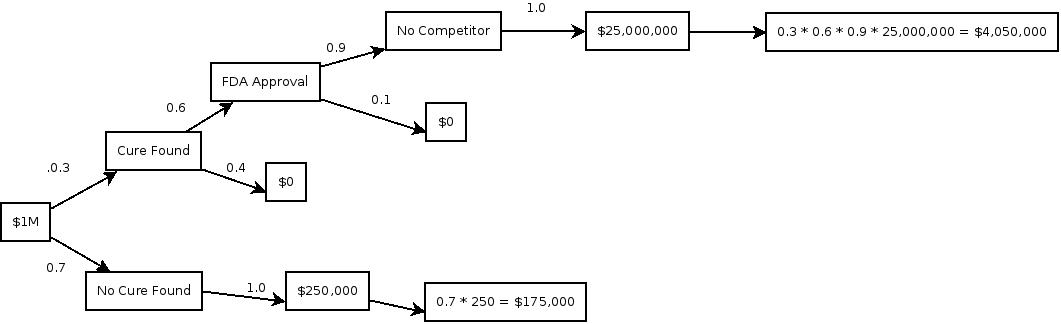
\includegraphics[scale = 0.25]{investment.jpeg}
    \caption{Investment Decision}
  \end{figure}

  \begin{solution}
    \begin{itemize*}
      \item There is a 0.7 chance of \$175,000 
      \item There is a 0.162 chance of \$4,050,000 
      \item There is a 0.138 chance of \$0
    \end{itemize*}
    
    \$4,050,000 + \$175,000 = \fbox{ \$4,225,000 }

    It's a good investment, as long as you can afford to invest in enough
    companies for the law of large numbers to take effect.

   \end{solution}

\end{document}

